\documentclass{standalone}
\usepackage{tikz}
\usetikzlibrary{patterns, positioning}
\usepackage[sfdefault]{ClearSans} %% option 'sfdefault' activates Clear Sans as the default text font
\usepackage[T1]{fontenc}

\begin{document}
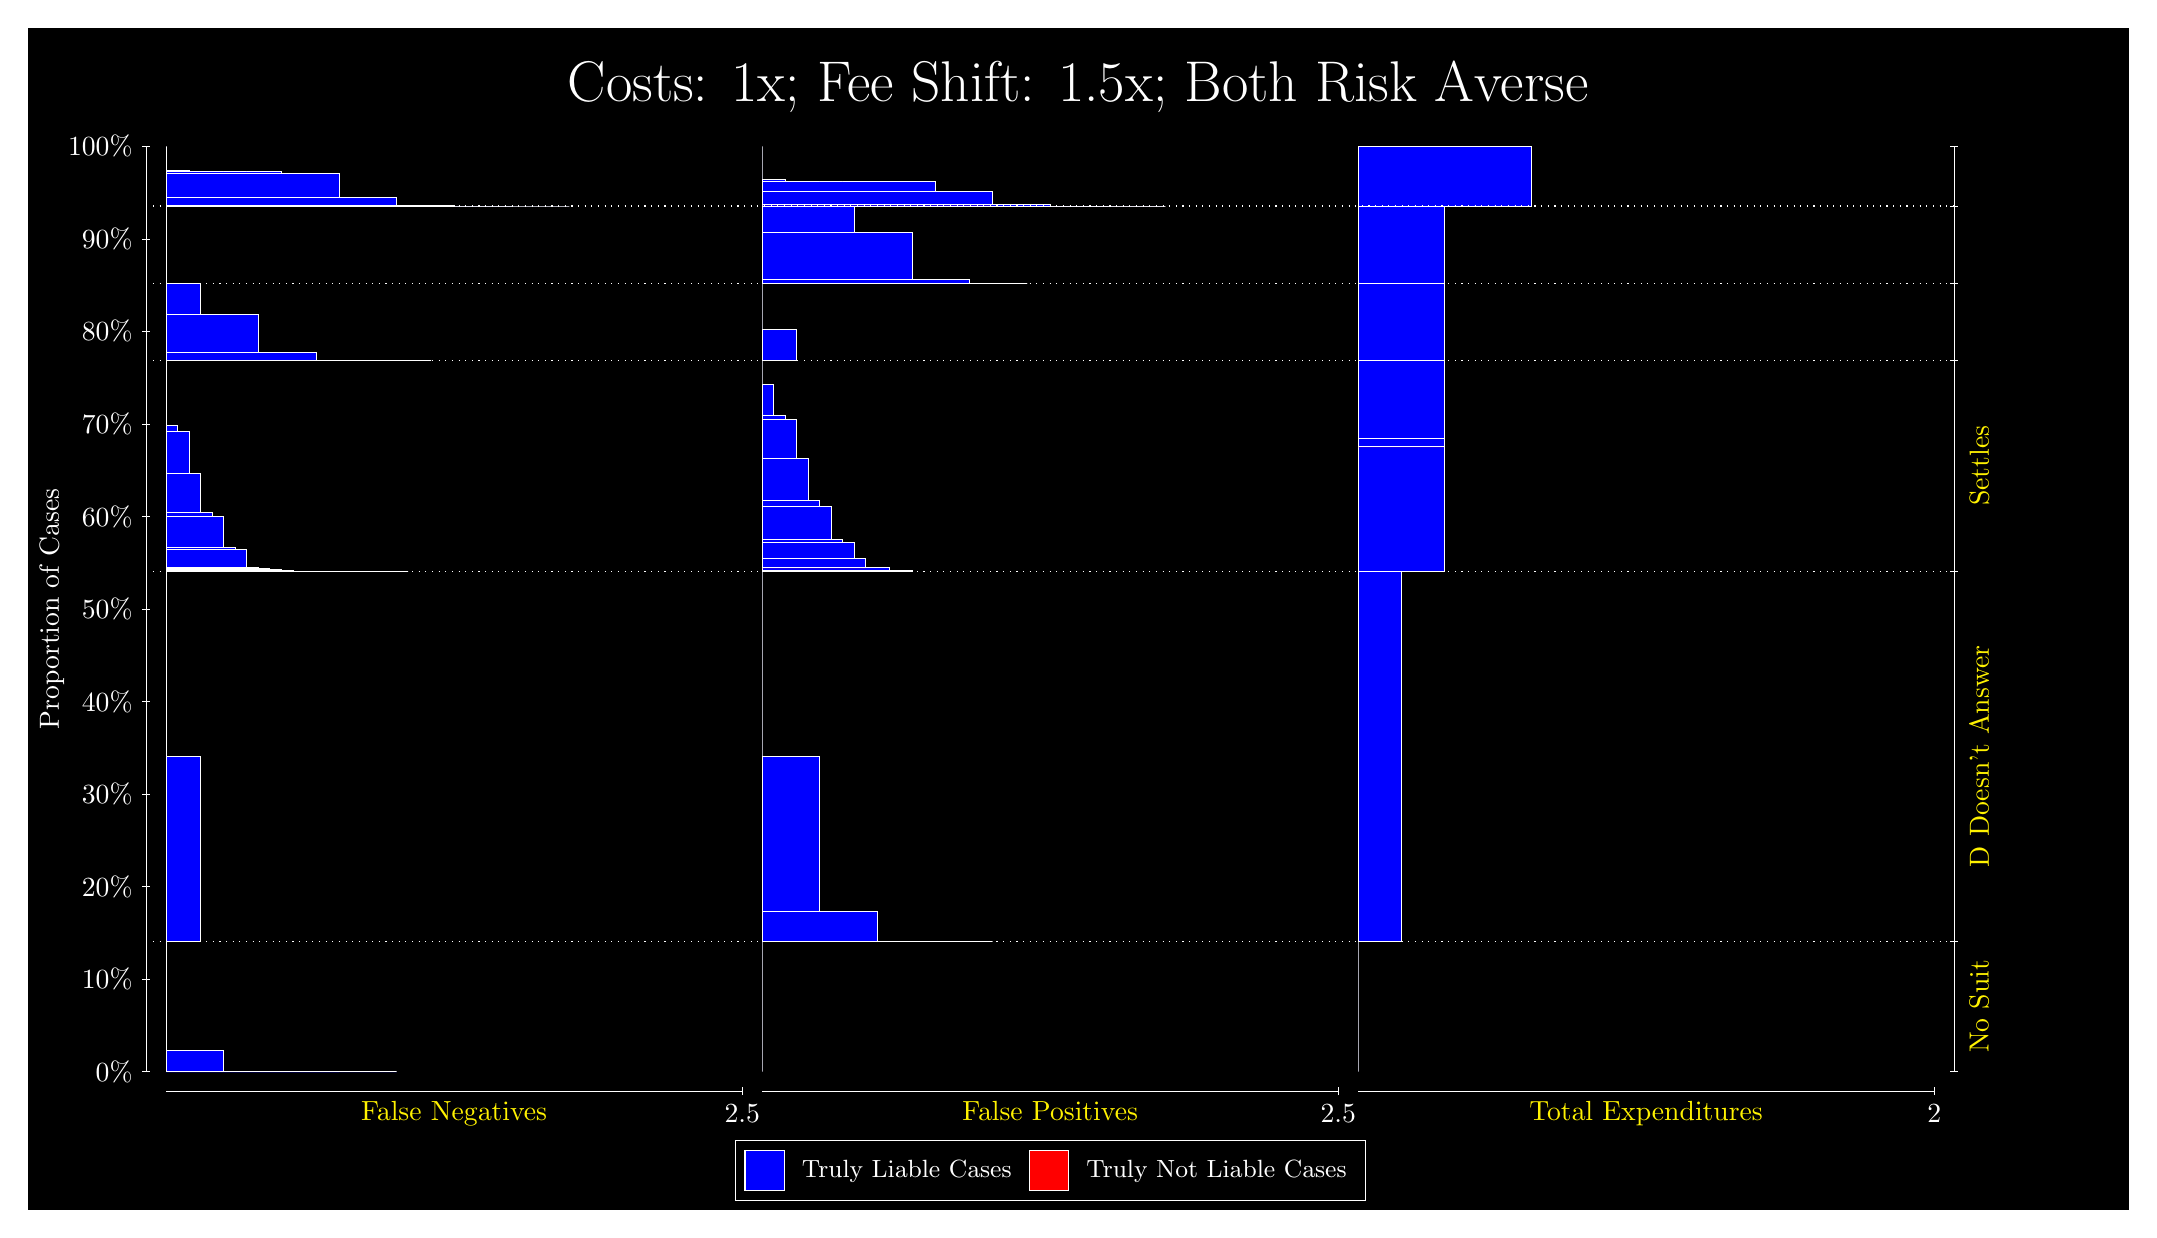
\begin{tikzpicture}
\draw[fill=black] (0,0) rectangle (26.667,15);
\draw[text=white] (0,13.5) rectangle (26.667,15) node[midway] {\huge Costs: 1x; Fee Shift: 1.5x; Both Risk Averse};
\draw[white, very thin] (1.5,1.75) -- (1.5,13.5);
\node[rotate=90, text=white, anchor=center] at (0.3, 7.625) {Proportion of Cases};
\draw[white, very thin] (1.45,1.75) -- (1.55,1.75);
\node[text=white, anchor=east] at (1.45, 1.75) {0\%};
\draw[white, very thin] (1.45,2.925) -- (1.55,2.925);
\node[text=white, anchor=east] at (1.45, 2.925) {10\%};
\draw[white, very thin] (1.45,4.1) -- (1.55,4.1);
\node[text=white, anchor=east] at (1.45, 4.1) {20\%};
\draw[white, very thin] (1.45,5.275) -- (1.55,5.275);
\node[text=white, anchor=east] at (1.45, 5.275) {30\%};
\draw[white, very thin] (1.45,6.45) -- (1.55,6.45);
\node[text=white, anchor=east] at (1.45, 6.45) {40\%};
\draw[white, very thin] (1.45,7.625) -- (1.55,7.625);
\node[text=white, anchor=east] at (1.45, 7.625) {50\%};
\draw[white, very thin] (1.45,8.8) -- (1.55,8.8);
\node[text=white, anchor=east] at (1.45, 8.8) {60\%};
\draw[white, very thin] (1.45,9.975) -- (1.55,9.975);
\node[text=white, anchor=east] at (1.45, 9.975) {70\%};
\draw[white, very thin] (1.45,11.15) -- (1.55,11.15);
\node[text=white, anchor=east] at (1.45, 11.15) {80\%};
\draw[white, very thin] (1.45,12.325) -- (1.55,12.325);
\node[text=white, anchor=east] at (1.45, 12.325) {90\%};
\draw[white, very thin] (1.45,13.5) -- (1.55,13.5);
\node[text=white, anchor=east] at (1.45, 13.5) {100\%};

\draw[white, very thin] (24.457,1.75) -- (24.457,13.5);
\draw[white, very thin] (24.407,1.75) -- (24.507,1.75);
\node[anchor=west] at (24.407, 1.75) {};
\draw[white, very thin] (24.407,3.4045) -- (24.507,3.4045);
\node[anchor=west] at (24.407, 3.4045) {};
\draw[white, very thin] (24.407,8.1027) -- (24.507,8.1027);
\node[anchor=west] at (24.407, 8.1027) {};
\draw[white, very thin] (24.407,10.783) -- (24.507,10.783);
\node[anchor=west] at (24.407, 10.783) {};
\draw[white, very thin] (24.407,11.761) -- (24.507,11.761);
\node[anchor=west] at (24.407, 11.761) {};
\draw[white, very thin] (24.407,12.742) -- (24.507,12.742);
\node[anchor=west] at (24.407, 12.742) {};
\draw[white, very thin] (24.407,13.5) -- (24.507,13.5);
\node[anchor=west] at (24.407, 13.5) {};

\draw[white, very thin, fill=blue] (1.75,1.75) rectangle (4.6775,1.75);
\draw[white, very thin, fill=blue] (1.75,1.75) rectangle (3.9457,1.75);
\draw[white, very thin, fill=blue] (1.75,1.75) rectangle (3.2138,1.7523);
\draw[white, very thin, fill=blue] (1.75,1.7523) rectangle (2.4819,2.0209);
\draw[white, very thin, fill=red] (1.75,2.0209) rectangle (1.75,2.0209);
\draw[white, very thin, fill=blue] (1.75,2.0209) rectangle (1.75,3.4045);
\draw[white, very thin, fill=blue] (1.75,3.4045) rectangle (2.1891,5.7507);
\draw[white, very thin, fill=red] (1.75,5.7507) rectangle (1.75,5.7507);
\draw[white, very thin, fill=blue] (1.75,5.7507) rectangle (1.75,8.1027);
\draw[white, very thin, fill=blue] (1.75,8.1027) rectangle (4.8239,8.1027);
\draw[white, very thin, fill=blue] (1.75,8.1027) rectangle (4.5312,8.1027);
\draw[white, very thin, fill=blue] (1.75,8.1027) rectangle (4.2384,8.1027);
\draw[white, very thin, fill=blue] (1.75,8.1027) rectangle (4.092,8.1027);
\draw[white, very thin, fill=blue] (1.75,8.1027) rectangle (3.9457,8.1027);
\draw[white, very thin, fill=blue] (1.75,8.1027) rectangle (3.7993,8.103);
\draw[white, very thin, fill=blue] (1.75,8.103) rectangle (3.6529,8.103);
\draw[white, very thin, fill=blue] (1.75,8.103) rectangle (3.5065,8.1091);
\draw[white, very thin, fill=blue] (1.75,8.1091) rectangle (3.3602,8.1098);
\draw[white, very thin, fill=blue] (1.75,8.1098) rectangle (3.2138,8.1226);
\draw[white, very thin, fill=blue] (1.75,8.1226) rectangle (3.0674,8.1373);
\draw[white, very thin, fill=blue] (1.75,8.1373) rectangle (2.921,8.1589);
\draw[white, very thin, fill=blue] (1.75,8.1589) rectangle (2.7746,8.3883);
\draw[white, very thin, fill=blue] (1.75,8.3883) rectangle (2.6283,8.4134);
\draw[white, very thin, fill=blue] (1.75,8.4134) rectangle (2.4819,8.7967);
\draw[white, very thin, fill=blue] (1.75,8.7967) rectangle (2.3355,8.8568);
\draw[white, very thin, fill=blue] (1.75,8.8568) rectangle (2.1891,9.3525);
\draw[white, very thin, fill=blue] (1.75,9.3525) rectangle (2.0428,9.8782);
\draw[white, very thin, fill=blue] (1.75,9.8782) rectangle (1.8964,9.9579);
\draw[white, very thin, fill=red] (1.75,9.9579) rectangle (1.75,9.9579);
\draw[white, very thin, fill=blue] (1.75,9.9579) rectangle (1.75,10.783);
\draw[white, very thin, fill=blue] (1.75,10.783) rectangle (5.1167,10.783);
\draw[white, very thin, fill=blue] (1.75,10.783) rectangle (4.3848,10.785);
\draw[white, very thin, fill=blue] (1.75,10.785) rectangle (3.6529,10.881);
\draw[white, very thin, fill=blue] (1.75,10.881) rectangle (2.921,11.367);
\draw[white, very thin, fill=blue] (1.75,11.367) rectangle (2.1891,11.761);
\draw[white, very thin, fill=red] (1.75,11.761) rectangle (1.75,11.761);
\draw[white, very thin, fill=blue] (1.75,11.761) rectangle (2.1891,11.765);
\draw[white, very thin, fill=red] (1.75,11.765) rectangle (1.75,11.765);
\draw[white, very thin, fill=blue] (1.75,11.765) rectangle (1.75,12.742);
\draw[white, very thin, fill=blue] (1.75,12.742) rectangle (6.8732,12.742);
\draw[white, very thin, fill=blue] (1.75,12.742) rectangle (6.1413,12.742);
\draw[white, very thin, fill=blue] (1.75,12.742) rectangle (5.4094,12.746);
\draw[white, very thin, fill=blue] (1.75,12.746) rectangle (4.6775,12.849);
\draw[white, very thin, fill=blue] (1.75,12.849) rectangle (3.9457,13.157);
\draw[white, very thin, fill=blue] (1.75,13.157) rectangle (3.5065,13.157);
\draw[white, very thin, fill=blue] (1.75,13.157) rectangle (3.2138,13.186);
\draw[white, very thin, fill=blue] (1.75,13.186) rectangle (2.7746,13.186);
\draw[white, very thin, fill=blue] (1.75,13.186) rectangle (2.7746,13.186);
\draw[white, very thin, fill=blue] (1.75,13.186) rectangle (2.4819,13.186);
\draw[white, very thin, fill=blue] (1.75,13.186) rectangle (2.0428,13.187);
\draw[white, very thin, fill=blue] (1.75,13.187) rectangle (2.0428,13.192);
\draw[white, very thin, fill=red] (1.75,13.192) rectangle (1.75,13.192);
\draw[white, very thin, fill=blue] (1.75,13.192) rectangle (1.75,13.5);
\draw[white, very thin, fill=red] (9.3189,1.75) rectangle (9.3189,1.75);
\draw[white, very thin, fill=blue] (9.3189,1.75) rectangle (9.3189,3.4045);
\draw[white, very thin, fill=red] (9.3189,3.4045) rectangle (12.246,3.4045);
\draw[white, very thin, fill=blue] (9.3189,3.4045) rectangle (12.246,3.4045);
\draw[white, very thin, fill=blue] (9.3189,3.4045) rectangle (11.515,3.4074);
\draw[white, very thin, fill=blue] (9.3189,3.4074) rectangle (10.783,3.7798);
\draw[white, very thin, fill=blue] (9.3189,3.7798) rectangle (10.051,5.7565);
\draw[white, very thin, fill=blue] (9.3189,5.7565) rectangle (9.3189,8.1027);
\draw[white, very thin, fill=red] (9.3189,8.1027) rectangle (11.222,8.1027);
\draw[white, very thin, fill=blue] (9.3189,8.1027) rectangle (11.222,8.1162);
\draw[white, very thin, fill=red] (9.3189,8.1162) rectangle (10.929,8.1162);
\draw[white, very thin, fill=blue] (9.3189,8.1162) rectangle (10.929,8.1488);
\draw[white, very thin, fill=red] (9.3189,8.1488) rectangle (10.636,8.1488);
\draw[white, very thin, fill=blue] (9.3189,8.1488) rectangle (10.636,8.2716);
\draw[white, very thin, fill=blue] (9.3189,8.2716) rectangle (10.49,8.4764);
\draw[white, very thin, fill=red] (9.3189,8.4764) rectangle (10.344,8.4764);
\draw[white, very thin, fill=blue] (9.3189,8.4764) rectangle (10.344,8.5084);
\draw[white, very thin, fill=blue] (9.3189,8.5084) rectangle (10.197,8.928);
\draw[white, very thin, fill=red] (9.3189,8.928) rectangle (10.051,8.928);
\draw[white, very thin, fill=blue] (9.3189,8.928) rectangle (10.051,9.0076);
\draw[white, very thin, fill=blue] (9.3189,9.0076) rectangle (9.9044,9.5333);
\draw[white, very thin, fill=blue] (9.3189,9.5333) rectangle (9.758,10.029);
\draw[white, very thin, fill=blue] (9.3189,10.029) rectangle (9.6116,10.089);
\draw[white, very thin, fill=blue] (9.3189,10.089) rectangle (9.4652,10.472);
\draw[white, very thin, fill=blue] (9.3189,10.472) rectangle (9.3189,10.783);
\draw[white, very thin, fill=red] (9.3189,10.783) rectangle (9.758,10.783);
\draw[white, very thin, fill=blue] (9.3189,10.783) rectangle (9.758,11.177);
\draw[white, very thin, fill=blue] (9.3189,11.177) rectangle (9.3189,11.761);
\draw[white, very thin, fill=red] (9.3189,11.761) rectangle (12.686,11.761);
\draw[white, very thin, fill=blue] (9.3189,11.761) rectangle (12.686,11.761);
\draw[white, very thin, fill=blue] (9.3189,11.761) rectangle (11.954,11.817);
\draw[white, very thin, fill=blue] (9.3189,11.817) rectangle (11.222,12.411);
\draw[white, very thin, fill=blue] (9.3189,12.411) rectangle (10.49,12.738);
\draw[white, very thin, fill=blue] (9.3189,12.738) rectangle (9.758,12.742);
\draw[white, very thin, fill=red] (9.3189,12.742) rectangle (14.442,12.742);
\draw[white, very thin, fill=blue] (9.3189,12.742) rectangle (14.442,12.742);
\draw[white, very thin, fill=red] (9.3189,12.742) rectangle (13.71,12.742);
\draw[white, very thin, fill=blue] (9.3189,12.742) rectangle (13.71,12.742);
\draw[white, very thin, fill=red] (9.3189,12.742) rectangle (12.978,12.742);
\draw[white, very thin, fill=blue] (9.3189,12.742) rectangle (12.978,12.761);
\draw[white, very thin, fill=red] (9.3189,12.761) rectangle (12.246,12.761);
\draw[white, very thin, fill=blue] (9.3189,12.761) rectangle (12.246,12.931);
\draw[white, very thin, fill=blue] (9.3189,12.931) rectangle (11.515,13.05);
\draw[white, very thin, fill=blue] (9.3189,13.05) rectangle (10.783,13.056);
\draw[white, very thin, fill=red] (9.3189,13.056) rectangle (10.344,13.056);
\draw[white, very thin, fill=blue] (9.3189,13.056) rectangle (10.344,13.056);
\draw[white, very thin, fill=blue] (9.3189,13.056) rectangle (10.051,13.056);
\draw[white, very thin, fill=red] (9.3189,13.056) rectangle (9.6116,13.056);
\draw[white, very thin, fill=blue] (9.3189,13.056) rectangle (9.6116,13.085);
\draw[white, very thin, fill=red] (9.3189,13.085) rectangle (9.3189,13.085);
\draw[white, very thin, fill=blue] (9.3189,13.085) rectangle (9.3189,13.5);
\draw[white, very thin, fill=red] (16.888,1.75) rectangle (16.888,1.75);
\draw[white, very thin, fill=blue] (16.888,1.75) rectangle (16.888,3.4045);
\draw[white, very thin, fill=red] (16.888,3.4045) rectangle (17.437,3.4045);
\draw[white, very thin, fill=blue] (16.888,3.4045) rectangle (17.437,8.1027);
\draw[white, very thin, fill=red] (16.888,8.1027) rectangle (17.986,8.1027);
\draw[white, very thin, fill=blue] (16.888,8.1027) rectangle (17.986,9.6865);
\draw[white, very thin, fill=red] (16.888,9.6865) rectangle (17.986,9.6865);
\draw[white, very thin, fill=blue] (16.888,9.6865) rectangle (17.986,9.7921);
\draw[white, very thin, fill=red] (16.888,9.7921) rectangle (17.986,9.7921);
\draw[white, very thin, fill=blue] (16.888,9.7921) rectangle (17.986,10.783);
\draw[white, very thin, fill=red] (16.888,10.783) rectangle (17.986,10.783);
\draw[white, very thin, fill=blue] (16.888,10.783) rectangle (17.986,11.761);
\draw[white, very thin, fill=red] (16.888,11.761) rectangle (17.986,11.761);
\draw[white, very thin, fill=blue] (16.888,11.761) rectangle (17.986,12.742);
\draw[white, very thin, fill=red] (16.888,12.742) rectangle (19.083,12.742);
\draw[white, very thin, fill=blue] (16.888,12.742) rectangle (19.083,13.5);
\draw[white, dotted] (1.5,3.4045) -- (24.457,3.4045);
\draw[white, dotted] (1.5,8.1027) -- (24.457,8.1027);
\draw[white, dotted] (1.5,10.783) -- (24.457,10.783);
\draw[white, dotted] (1.5,11.761) -- (24.457,11.761);
\draw[white, dotted] (1.5,12.742) -- (24.457,12.742);
\draw[white, very thin] (1.75,1.5) -- (9.0689,1.5);
\node[text=yellow, anchor=north] at (5.4094, 1.5) {False Negatives};
\draw[white, very thin] (9.0689,1.45) -- (9.0689,1.55);
\node[text=white, anchor=north] at (9.0689, 1.45) {2.5};

\draw[white, very thin] (9.3189,1.5) -- (16.638,1.5);
\node[text=yellow, anchor=north] at (12.978, 1.5) {False Positives};
\draw[white, very thin] (16.638,1.45) -- (16.638,1.55);
\node[text=white, anchor=north] at (16.638, 1.45) {2.5};

\draw[white, very thin] (16.888,1.5) -- (24.207,1.5);
\node[text=yellow, anchor=north] at (20.547, 1.5) {Total Expenditures};
\draw[white, very thin] (24.207,1.45) -- (24.207,1.55);
\node[text=white, anchor=north] at (24.207, 1.45) {2};

\node[text=yellow, centered, rotate=90] at (24.777, 2.5773) {No Suit};
\node[text=yellow, centered, rotate=90] at (24.777, 5.7536) {D Doesn't Answer};
\node[text=yellow, centered, rotate=90] at (24.777, 9.4429) {Settles};




\draw (12.978300999999998,1.5) node[draw=none] (baseCoordinate) {};
\begin{scope}[align=center]
        \matrix[scale=0.5, draw=white, below=0.5cm of baseCoordinate, nodes={draw}, column sep=0.1cm]{
            \node[rectangle, draw, minimum width=0.5cm, minimum height=0.5cm, fill=blue] {}; &
            \node[draw=none, font=\small, text=white] (B) {Truly Liable Cases}; &
            \node[rectangle, draw, minimum width=0.5cm, minimum height=0.5cm, fill=red] {}; &
            \node[draw=none, font=\small, text=white] (B) {Truly Not Liable Cases}; \\
            };
\end{scope}

\end{tikzpicture}
\end{document}